\chapter{Estado del Arte}\label{chapter: sota}

Con el incremento constante de la cantidad de información generada en todo el mundo, la recuperación de información se ha convertido en un aspecto de creciente relevancia tanto en el ámbito industrial como en el académico. En consecuencia, la reducción del tiempo transcurrido entre el momento en que un usuario desea acceder a la información y el momento en que efectivamente puede hacerlo ha sido objeto de un número creciente de investigaciones científicas en los últimos años. Este capítulo se dedica a la evaluación de diversas estructuras de interfaces entre el ser humano y bases de conocimiento, las cuales tienen como objetivo abordar esta problemática.

Las Interfaces de Lenguaje Natural a Bases de Datos (NLIDB, por sus siglas en inglés) representan un campo de investigación dinámico centrado en facilitar las interacciones entre humanos y computadoras con bases de datos relacionales utilizando consultas en lenguaje natural. A lo largo de las últimas décadas, el desarrollo de NLIDB ha pasado por varias fases transformadoras, impulsadas por avances tecnológicos y metodológicos, así como por una creciente demanda de una mejor accesibilidad a las bases de datos.

Las etapas iniciales del desarrollo de NLIDB se caracterizaron por sistemas específicos de dominio. Estos sistemas fueron diseñados para trabajar dentro de áreas de conocimiento bien definidas, donde se utilizaba el procesamiento de lenguaje natural controlado para garantizar la comprensión de las consultas y la interacción con la base de datos. Por ejemplo, algunos trabajos pioneros \cite{popescuetal2003} \cite{popescuetal2004} demostraron NLIDBs que se adaptaban a dominios específicos, lo que los hacía altamente efectivos pero limitados en alcance. Del mismo modo, en años posteriores \cite{lietal2007} \cite{liandjagadish2014} se continuó la exploración del uso de interfaces de lenguaje natural controlado dentro de dominios de conocimiento particulares.

Otro enfoque durante esta fase implicó NLIDBs basados en reglas. Algunos sistemas propuestos al respecto \cite{straticaetal2005} dependían de reglas predefinidas para traducir consultas en lenguaje natural en declaraciones \textit{SQL} para la recuperación de datos en la base de datos. Si bien estos sistemas ofrecían ciertas ventajas, carecían de versatilidad para manejar una amplia gama de consultas de usuarios en diferentes dominios.

A medida que avanzaba la investigación en NLIDB, hubo un cambio hacia la independencia de dominio y la flexibilidad. Los sistemas recientes han buscado reducir la dependencia del conocimiento específico del dominio y las reglas. Algunos investigadores \cite{zhongetal2017} \cite{yuetal2018}) han desarrollado NLIDBs que utilizan técnicas de aprendizaje supervisado, lo que los hace más adaptables a varios dominios y entradas de usuario. Además, un avance significativo se ha producido con la integración de redes neuronales profundas en el desarrollo de NLIDBs, donde varias investigaciones \cite{dongandlapata2016} \cite{devlinetal2018} han demostrado el potencial del aprendizaje profundo en NLIDB, aprovechando vastos repositorios de texto y código para el entrenamiento. Este enfoque ha mejorado significativamente el rendimiento de NLIDB, permitiendo un procesamiento de consultas más natural y contextual.

Para el caso específico de NLIDB con respecto a BDOGs inicialmente se desarrollaron trabajos enfocados en técnicas similares a las empleadas para \textit{SQL} \cite{adrainbazaga2021} \cite{hainsetal2019}, donde se realizaba un preprocesamiento en la consulta dada, se aprovechaba la información ofrecida por el esquema \cite{dbschema} de la base de datos a consultar y finalmente dicho conocimiento era utilizado por un modelo de aprendizaje profundo entrenado sobre un conjunto de pares de lenguaje natural y lenguaje de consulta formal como por ejemplo \textit{Cypher}.

Recientemente, los trabajos orientados a esta área de estudio han estado enfocados en dos metodologías principales:
\begin{enumerate}
	\item Enfoques neurosimbólicos basados en representación intermedia de la consulta dada en lenguaje natural.
	\item Enfoques basados en técnicas de \textit{prompt engineering} mediante LLMs.
\end{enumerate}

\section{Enfoques neurosimbólicos basados en representación intermedia (IR, por sus siglas en inglés) de la consulta dada en lenguaje natural} \label{neurosymbolic_approach}

Con respecto a la recuperación de información de una base de conocimiento con este enfoque, mediante consultas hechas en lenguaje natural se han hecho varias investigaciones científicas que se pueden agrupar bajo el patrón de la Figura \ref{neurosym_approach}.

\begin{figure*}[!h]\label{neurosym_approach}
	\centering
	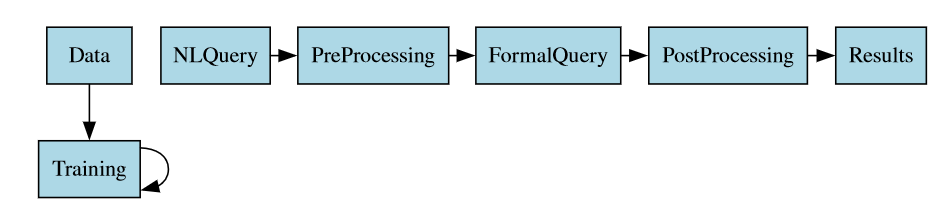
\includegraphics[width = 0.9\textwidth]{./Graphics/neurosym_approach}
	\caption{Secuencia de flujo representativa del Estado del Arte de traducción de
Lenguaje Natural a Lenguaje Formal utilizando el enfoque neurosimbólico basado en (IR).}
\end{figure*}

\subsection{Conjuntos de entranamiento y evaluación} \label{neurosymbolic_approach_bechmarks}

En cuanto a los datos para el entrenamiento existen dos opciones. Básicamente se puede buscar un conjunto de datos de referencia(\textit{Benchmark}) en los que entrenar y probar el sistema, o se crea uno. La mayoría de las investigaciones existentes elijen la primera opción. Algunos de los \textit{Benchmarks} más populares son:

\begin{itemize}
	\item \textbf{WikiSQL}: WikiSQL \cite{wikisql} es el banco de datos más grande y más utilizado, contiene $26531$ tablas y $80654$ pares de consultas en lenguaje natural y lenguaje \textit{SQL}. Las tablas se extraen de tablas \textit{HTML} de Wikipedia. Luego, cada consulta en \textit{SQL} se genera automáticamente para una determinada tabla bajo la restricción de que la consulta produce un conjunto de resultados no vacío.

	\item \textbf{Spider}:	 Este \textit{Benchmark} \cite{spiderdataset} es un punto de referencia multidominio a gran escala con 200 bases de datos de 138 dominios diferentes y 10.181 pares de consultas.

	\item \textbf{MetaQA}: El conjunto de datos METAQA-Cypher, originalmente conocido como METAQA \cite{zhangetal2018}, contiene más de $400000$ pares de preguntas y respuestas de múltiples pasos obtenidos de la base de conocimiento WikiMovies \cite{milleretal2016}. Mientras que investigaciones previas se han centrado principalmente en la anotación SPARQL \cite{huangetal2021}, nuestra innovación implica reconfigurar METAQA en \textit{Cypher}, estableciéndolo como un valioso punto de referencia para el aprendizaje de pocos ejemplos.

\end{itemize}

En el caso alternativo, se suelen usar las propias bases de conocimiento objeto de
estudio para crear un conjunto de entrenamiento. Una de las técnicas empleadas para
esto es Random Walk \cite{randomwalk}, en la que se hace un recorrido aleatorio sobre un subconjunto de las entidades y relaciones de la base de conocimiento, y se elaboran consultas artificiales que respondan a dichas entidades y relaciones \cite{dominikopitz2022}.

\subsection{Preprocesamiento} \label{neurosym_approach_preprocessing}

En general las investigaciones en el área realizan algún tipo de preprocesamiento
a la consulta. Algunos realizan parafraseo para llevar la consulta a representaciones
canónicas \cite{canonical}, en su lugar otros realizan un análisis morfológico léxico, con toquenización, lematización, eliminación de stopwords, tagueo de partes de la oración (\textit{POS-taguing}), etc. \cite{postaguing}. También se encuentran las investigaciones que usan en esta etapa traducciones basadas en diccionarios especializados en el dominio, o de propósito general, al igual que ontologías, para "suavizar" vocablos difíciles de entender por el resto del sistema \cite{smoothhardwords}. Además se usan técnicas como vectorización de palabras (\textit{word2vector}), y transformación de la consulta a una representación en grafos \cite{word2vector}.

\subsection{Postprocesamiento} \label{neurosym_approach_postprocessing}

En la fase de Post-Procesamiento, se observan diversas enfoques en las investigaciones. La mayoría de los investigadores realizan un análisis semántico que implica la clasificación según tipos de datos, el uso de ontologías y bases de conocimiento externas para realizar mapeos \cite{postprocessing1} \cite{postprocessing2}. Algunos optan por convertir la consulta en una representación canónica, mientras que otros la transforman en un lenguaje intermedio antes de transpilarla al lenguaje objetivo \cite{postprocessing3}. También hay quienes la codifican directamente en forma de grafo, y algunos la convierten en embeddings \cite{postprocessing4}.

\subsection{Consulta} \label{neurosym_approach_query}

En la fase de construcción de la consulta, existen tres enfoques principales. El primero es un enfoque manual que implica la búsqueda y formateo de palabras clave como \textit{"where"} y \textit{"select"}, además del mapeo de atributos a tablas \cite{neurosymquery1}. Otra vía se centra en el uso de modelos, incluyendo decodificadores y en algunos casos redes neuronales convolucionales \cite{neurosymquery2}. También se emplea la construcción de la consulta formal mediante un compilador, especialmente cuando se ha utilizado un lenguaje intermedio entre el lenguaje natural y el formal de consulta\cite{neurosymquery3}.

\section{Enfoques basados en técnicas de \textit{prompt engineering} mediante LLMs} \label{llm_approach}

Con la creciente atención dada a los modelos de lenguaje a gran escala, estos se han convertido en un componente esencial en el procesamiento del lenguaje natural. A medida que aumenta el tamaño de los modelos preentrenados, también está cambiando gradualmente su uso. A diferencia de modelos como BERT \cite{devlinetal2018} y T5 \cite{raffeletal2020}, que requieren un proceso de entrenamiento con una pequeña cantidad de datos, modelos como GPT-3 \cite{brownetal2020} requieren un diseño de un texto de entrada para generar resultados deseados. El reciente modelo de \textit{ChatGPT} \cite{chatgpt}, que emplea Aprendizaje por Reforzamiento para la Retroalimentación Humana (RLHF) \cite{christianoetal2021}, simplifica el diseño de textos de entrada de calidad, lo que permite una mejor utilización de la capacidad de ZSL de modelos preentrenados a gran escala de manera conversacional. Debido a la sólida capacidad de dichos en la generación de código \cite{llmcodegenerationsample} y al hecho de que los modelos de generación de código suelen requerir una gran cantidad de datos anotados para producir buenos resultados \cite{codegenmodeldataamount}, un modelo de generación de código de ZSL se considera fundamental.

Para la tarea específica de generar código de un lenguaje de consulta formal como \textit{SQL} y \textit{Cypher} se han utilizado distintos enfoques basados en varias de las principales técnicas de \textit{prompt engineering}.

\subsection{Zero-Shot Learning} \label{llm_approach_zsl}
	Esta técnica se enfoca en la capacidad de un modelo para comprender y generar código en un lenguaje de consulta sin requerir ejemplos específicos de entrenamiento en ese lenguaje en particular. En otras palabras, el modelo puede realizar esta tarea "desde cero", sin conocimiento previo del lenguaje. Algunos estudio interesantes se han realizado principalmente en la tarea de traducir lenguaje natural a lenguaje \textit{SQL} \cite{text2sqlzsl1} \cite{text2sqlzsl2}, los cuales permiten inferir la calidad mínima que estos modelos pueden alcanzar en la realización de dicha tarea \cite{zslislowerbound}.

\begin{figure}[H]\label{zslpromtpsql}
	\centering
	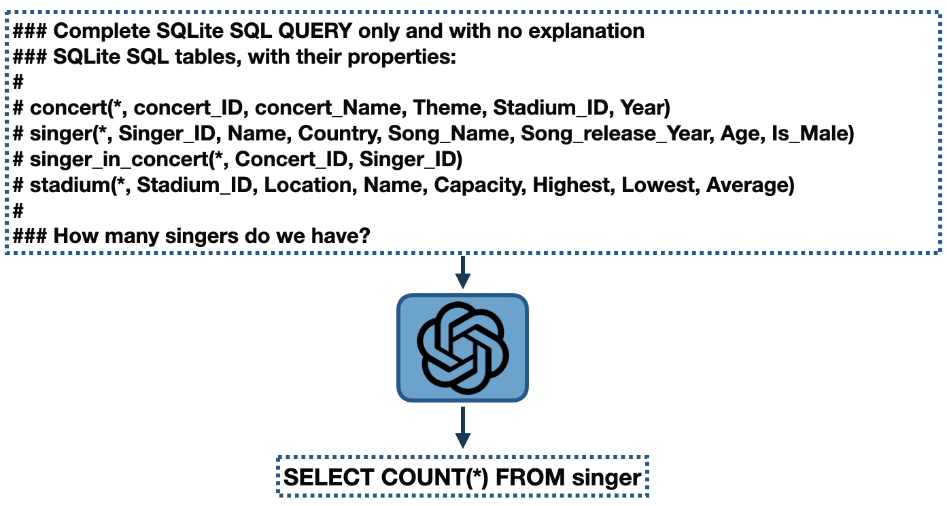
\includegraphics[width = 0.9\textwidth]{./Graphics/zslpromptsql}
	\caption{Ejemplo del flujo de trabajo de experimentos basados en ZSL para la traducción de lenguaje natural a código en \textit{SQL}.}
\end{figure} 

\subsection{Few-Shot Learning} \label{llm_approach_fsl}
	En contraste, el enfoque de Few-Shot Learning (FSL) se basa en la idea de que el modelo tiene acceso a un pequeño número de ejemplos (pocos ejemplos) en el lenguaje de consulta deseado para mejorar su capacidad de generar código en ese lenguaje. Esto puede ser especialmente útil cuando se necesita una adaptación rápida a un nuevo lenguaje o contexto. Tal y como muestran algunos resultados experimentales, este enfoque puede tener resultados superiores a varios modelos basados en \textit{fine-tuning} \cite{ftvsllmtext2sql}.

Un ejemplo notable de esta aplicación es el modelo Codex \cite{Codex}, que ha demostrado ser un fuerte baseline en el \textit{benchmark} Spider sin ninguna fase de entrenamiento. Además, se ha observado que proporcionar un pequeño número de ejemplos en el dominio en el prompt permite a Codex superar a los modelos de estado del arte cuyos parámetros han sido ajustados con pocos ejemplos de pocos dominios \cite{Codexresults}.

Además, se ha propuesto un marco de selección de demostraciones ODIS \cite{ODIS} que utiliza tanto ejemplos fuera de dominio como ejemplos generados sintéticamente en el dominio para construir demostraciones. Este enfoque ha demostrado ser efectivo en comparación con los métodos de línea de base que se basan en una única fuente de datos \cite{ODISresults}.

En cuanto a los conjuntos de datos, existen varios conjuntos de datos de texto a SQL que han sido propuestos para evaluar el rendimiento de los modelos LLM. Algunos de estos conjuntos de datos incluyen CoSQL, TableQA, DuSQL, CHASE, y BIRD-SQL \cite{wikisql} \cite{CoSQL} \cite{TableQA} \cite{DuSQL} \cite{CHASE} \cite{BIRD-SQL}.

\begin{figure}[H]\label{fslpromtpsql}
	\centering
	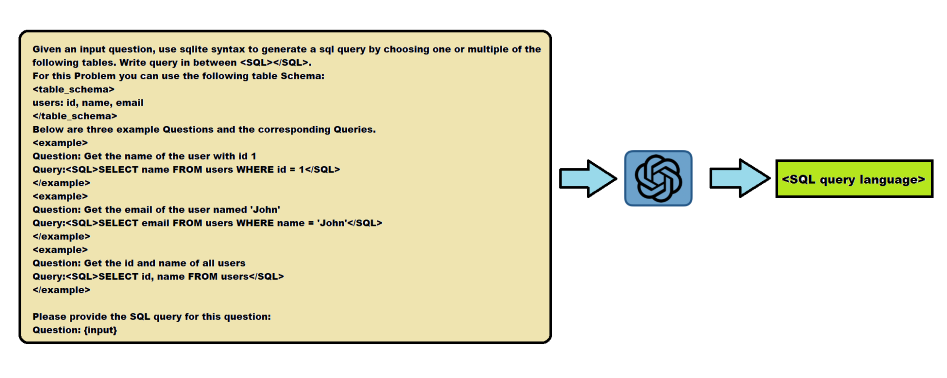
\includegraphics[width = 1\textwidth]{./Graphics/fslpromptsql}
	\caption{Ejemplo del flujo de trabajo de experimentos basados en FSL para la traducción de lenguaje natural a código en \textit{SQL}.}
\end{figure}

\subsection{Chain-of-Thought Prompting} \label{llm_approach_cot}

El enfoque de la cadena de pensamiento (\textit{Chain of Thought, CoT}) \cite{cot} en la conversión de texto a \textit{SQL} ha demostrado ser una estrategia prometedora para mejorar la capacidad de los modelos de lenguaje de gran tamaño (LLMs) para realizar razonamientos complejos. Este enfoque se ha utilizado en varias investigaciones recientes para mejorar la capacidad de los LLMs para realizar tareas de razonamiento complejo, como la conversión de texto a SQL \cite{cotllmssql1}.

Un estudio propuso un nuevo paradigma para la generación de consultas \textit{SQL} a partir de texto, llamado \textit{Divide-and-Prompt}, que divide la tarea en subtareas y luego aborda cada subtarea a través de la cadena de pensamiento. Se presentaron tres métodos basados en la indicación para mejorar la capacidad de los LLMs para generar consultas \textit{SQL} a partir de texto. Los experimentos mostraron que estas indicaciones guían a los LLMs para generar consultas \textit{SQL} a partir de texto con mayor precisión de ejecución \cite{cotllmssql2}.

\begin{figure}[H]\label{fslpromtpsql}
	\centering
	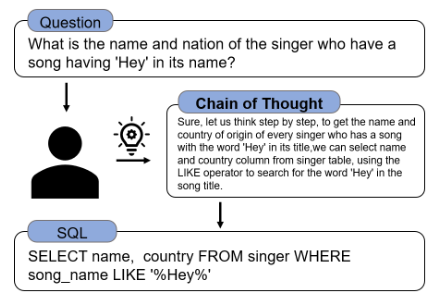
\includegraphics[width = 0.8\textwidth]{./Graphics/cotpromptsql}
	\caption{Ejemplo del flujo de trabajo de experimentos basados en CoT para la traducción de lenguaje natural a código en \textit{SQL}.}
\end{figure}

\subsection{\textit{Fine-Tuning}} \label{llm_approach_finetunig}

El entrenamiento (\textit{fine-tuning}) de un modelo es un proceso que se utiliza para mejorar el rendimiento de un modelo de aprendizaje automático en una tarea específica. En el contexto de la conversión de texto a \textit{SQL}, el ajuste fino puede ser utilizado para mejorar la precisión y la eficacia de los modelos de lenguaje de gran tamaño (LLMs) en la generación de consultas \textit{SQL} a partir de texto. Se han realizado estudios \cite propuso un método de \textit{fine-tuning} para los modelos LLMs utilizando un conjunto de datos de texto a \textit{SQL}, donde el método principal consistía en entrenar el modelo en el conjunto de datos de entrenamiento y luego ajustar el modelo en un conjunto de datos que contenía consultas \textit{SQL} generadas por humanos. Este método demostró ser efectivo para mejorar la precisión de los modelos LLMs en la generación de consultas \textit{SQL} a partir de texto \cite{finetuningtext2sql}.

Este enfoque constituye una poderosa herramienta  en la conversión de lenguaje natural a \textit{SQL}. Sin embargo, no es una solución mágica, ya que pocas organizaciones tienen conjuntos de datos de entrenamiento \textit{NL-2-SQL} disponibles de manera inmediata. Algunos expertos consideran que las mejores arquitecturas se podrían lograr combinando modelos ajustados con agentes RAG (\textit{Retrieval Augmented Generation}) \cite{raginfo}.

\section{Consideraciones generales} \label{llm_approach_finetunig}

A pesar del uso comprobado de dichos enfoques, todavía existe una escasez de estudios orientados a la traducción de lenguaje natural a código de consulta a BDOG como por ejemplo \textit{Cypher} \cite{gpt4graphpaper2023}, por lo tanto, es visible la necesidad de elaborar experimentos enfocados en dicha tarea, tomando como bases las ideas anteriormente expuestas.


%\newpage